\chapter{Alguns exemplos de comandos \LaTeX{}}
\label{chap:exemplos}

\section{Bibliografia e Referências}

A documentação do pacote biblatex\index{biblatex} é bastante extensa e explica
os diversos tipos de documento suportados, bem como o significado
de cada campo. Na prática, às vezes é preciso fazer escolhas sobre
o que incluir na descrição de um item bibliográfico e muitas vezes
é mais fácil aprender copiando exemplos já existentes, como estes (consulte o
arquivo \texttt{bibliografia.bib} para ver como foi criado o banco de dados e a
bibliografia na página \pageref{bibliografia} para ver o resultado impresso):

\begin{multicols}{2}
  \begin{itemize}
    \item @Book: \cite{JW82}.

    \item @Article: \cite{MenaChalco08}.

    \item @InProceedings: \cite{alves03:simi}.

    \item @Conference (sinônimo de @InProceedings): \cite{bronevetsky02}.

    \item @InCollection: \cite{bobaoglu93:concepts}.

    \item @PhdThesis: \cite{garcia01:PhD}.

    \item @MastersThesis: \cite{schmidt03:MSc}.

    \item @Techreport: \cite{alvisi99:analysisCIC}.

    \item @Manual: \cite{CORBA:spec}.

    \item @Misc: \cite{gridftp}.

    \item @Online (para referência a artigo \emph{online}): \cite{fowler04:designDead}.

    \item @Online (para referência a página web): \cite{FSF:GNU-GPL}.
  \end{itemize}
\end{multicols}

\section{Modo Matemático}\index{Modo Matemático}

O modo matemático do \LaTeX{} tem sintaxe própria, mas ela não é complicada e
há bastante documentação \emph{online} a respeito. Por exemplo, ``massa e
energia são grandezas relacionadas pela Equação $E=mc^2$, definida inicialmente
por Einstein'', ou ainda ``equações de segundo grau (Equação \ref{eq:2grau})
são estudadas no ensino médio. As raízes de uma equação de segundo grau podem
ser encontradas por~\eqref{eq:bhaskara} --- a fórmula de Bháskara.
O valor do discriminante $\Delta$ (Equação \ref{eq:delta}) determina se a
equação tem zero, uma ou duas raízes reais''. Observe que, quando um
parágrafo termina com um símbolo, pode ser boa ideia usar um espaço
não-separável (com ``\textsf{\textasciitilde}'') para evitar que ele
fique sozinho na última linha (por exemplo, ``\textsf{O discriminante é
denotado por\textasciitilde{}\$\textbackslash{}Delta\$}'').\label{orphanchar}

\begin{equation}
  \label{eq:2grau}
  ax^2+bx+c=y \quad \forall x \in \mathbb{R}
\end{equation}

\begin{gather}
\label{eq:bhaskara}
    y=0 \Leftrightarrow x=\frac{-b \pm \sqrt{\Delta}}{2a}
    \Leftrightarrow x \text{ é raiz da equação}\\
\label{eq:delta}
    \Delta\enspace(\mathit{delta}) = b^2-4ac
\end{gather}

\section{\emph{Floats} (Tabelas e Figuras)}\index{Floats}

Evidentemente, \LaTeX{} permite inserir figuras no texto; além
disso, ele também permite girá-las e criar subfiguras
(com sublegendas\index{Legendas}), como no exemplo da
Figura~\ref{fig:subfigures}\index{Subfiguras}, que inclui as
subfiguras \ref{fig:subfigures:a} e \ref{fig:subfigures:b}.
Uma ``figura'', na verdade, pode ser qualquer tipo de conteúdo
ilustrativo (como no caso da Figura~\ref{fig:gantt}, que é
um cronograma) mas, com a \textit{package} \textsf{float}, é
possível definir ambientes específicos para cada tipo de
conteúdo adicional (cada um com numeração independente), como
é o caso do Programa~\ref{prog:java}.\index{Floats}

% As packages relevantes para lidar com figuras são graphicx,
% float, caption, rotating e subcaption. Observe que "subfigure"
% e "subtable" são definidos na package subcaption, *não* na
% package subfigure! A package subfigure é obsoleta.

\begin{figure}
  \centering

  \begin{subfigure}{0.4\textwidth}
    \centering
    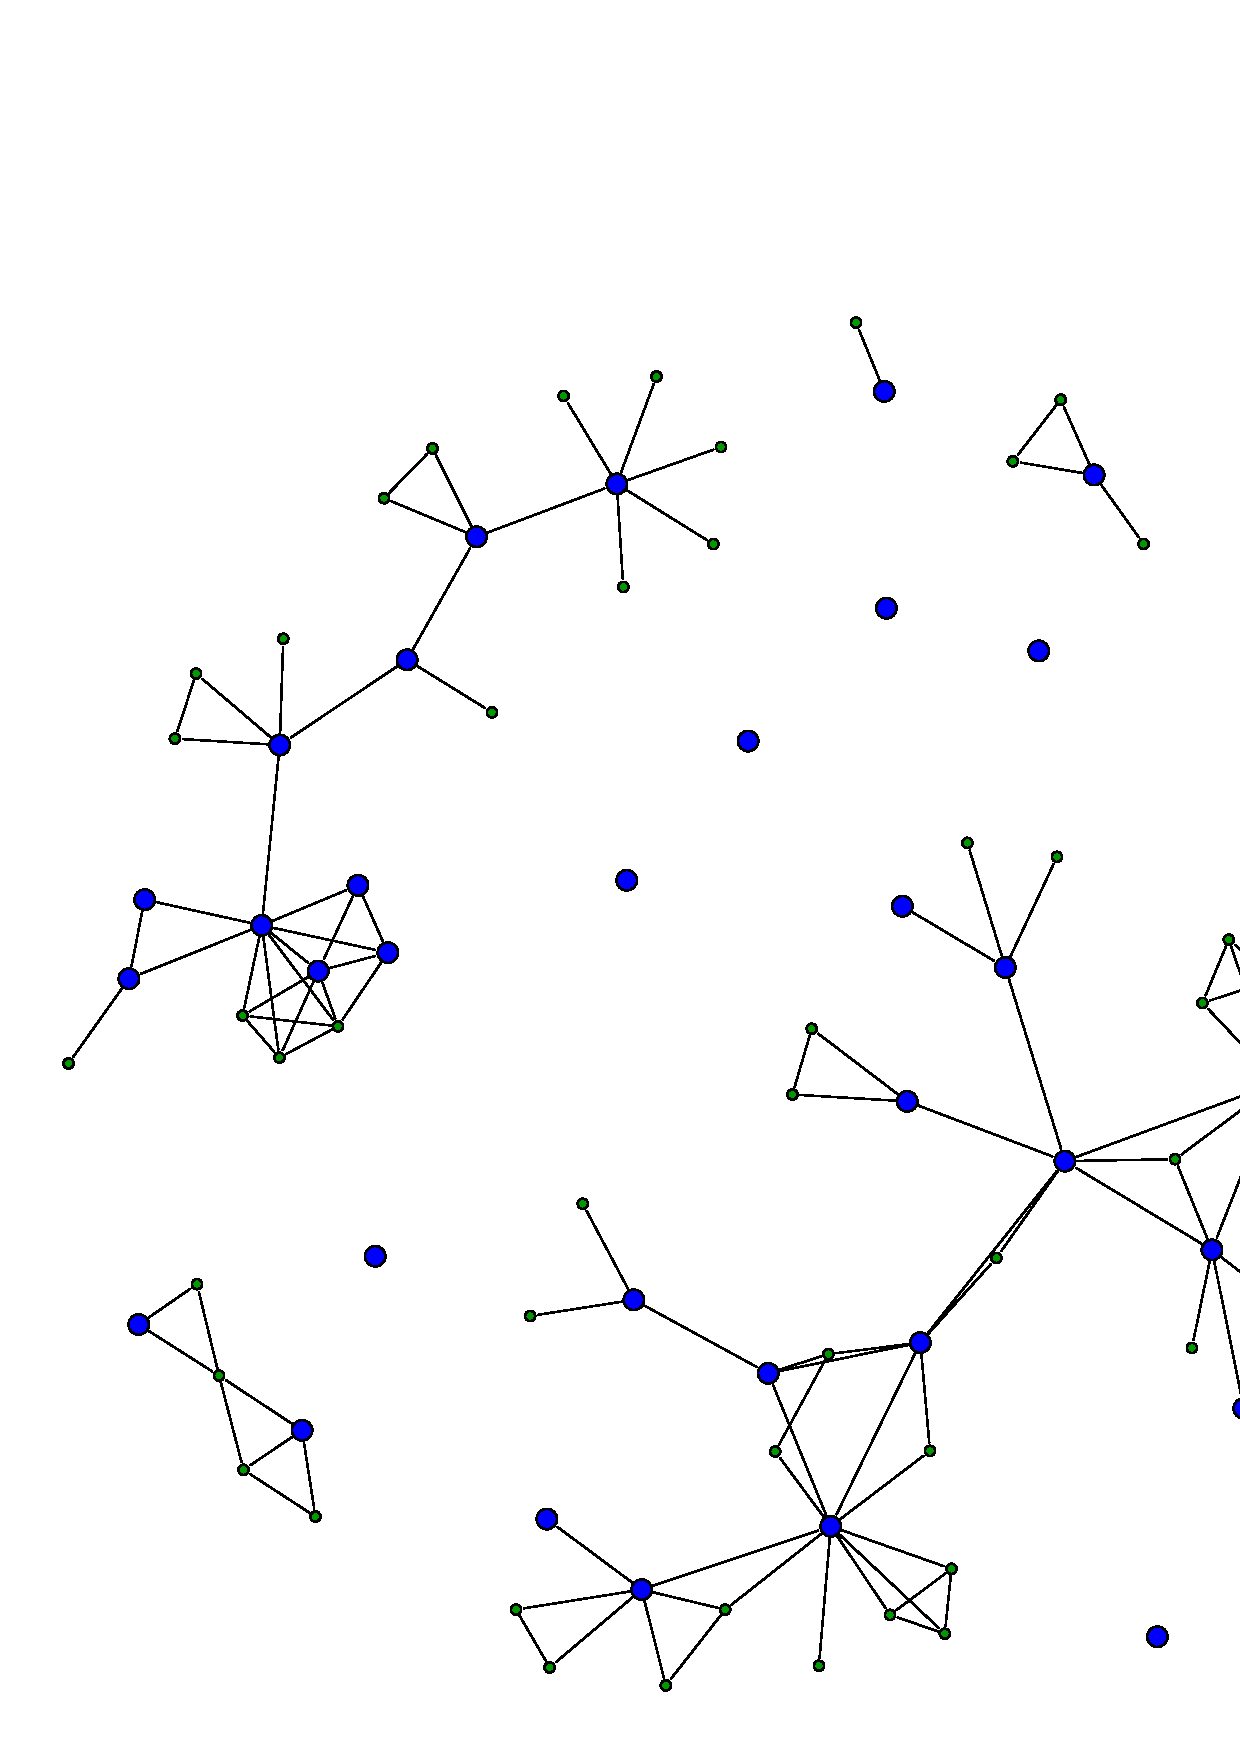
\includegraphics[width=.7\textwidth]{graph}
    \caption{Uma figura simples.}
    \label{fig:subfigures:a}
  \end{subfigure}
  % ATENÇÃO: Se você deixar uma linha em branco entre as subfiguras,
  % LaTeX vai considerar que cada uma delas pertence a um "parágrafo"
  % diferente e, portanto, vai colocá-las em linhas separadas ao invés
  % de lado a lado.
  \begin{subfigure}{0.4\textwidth}
    \centering
    \begin{turn}{90}
      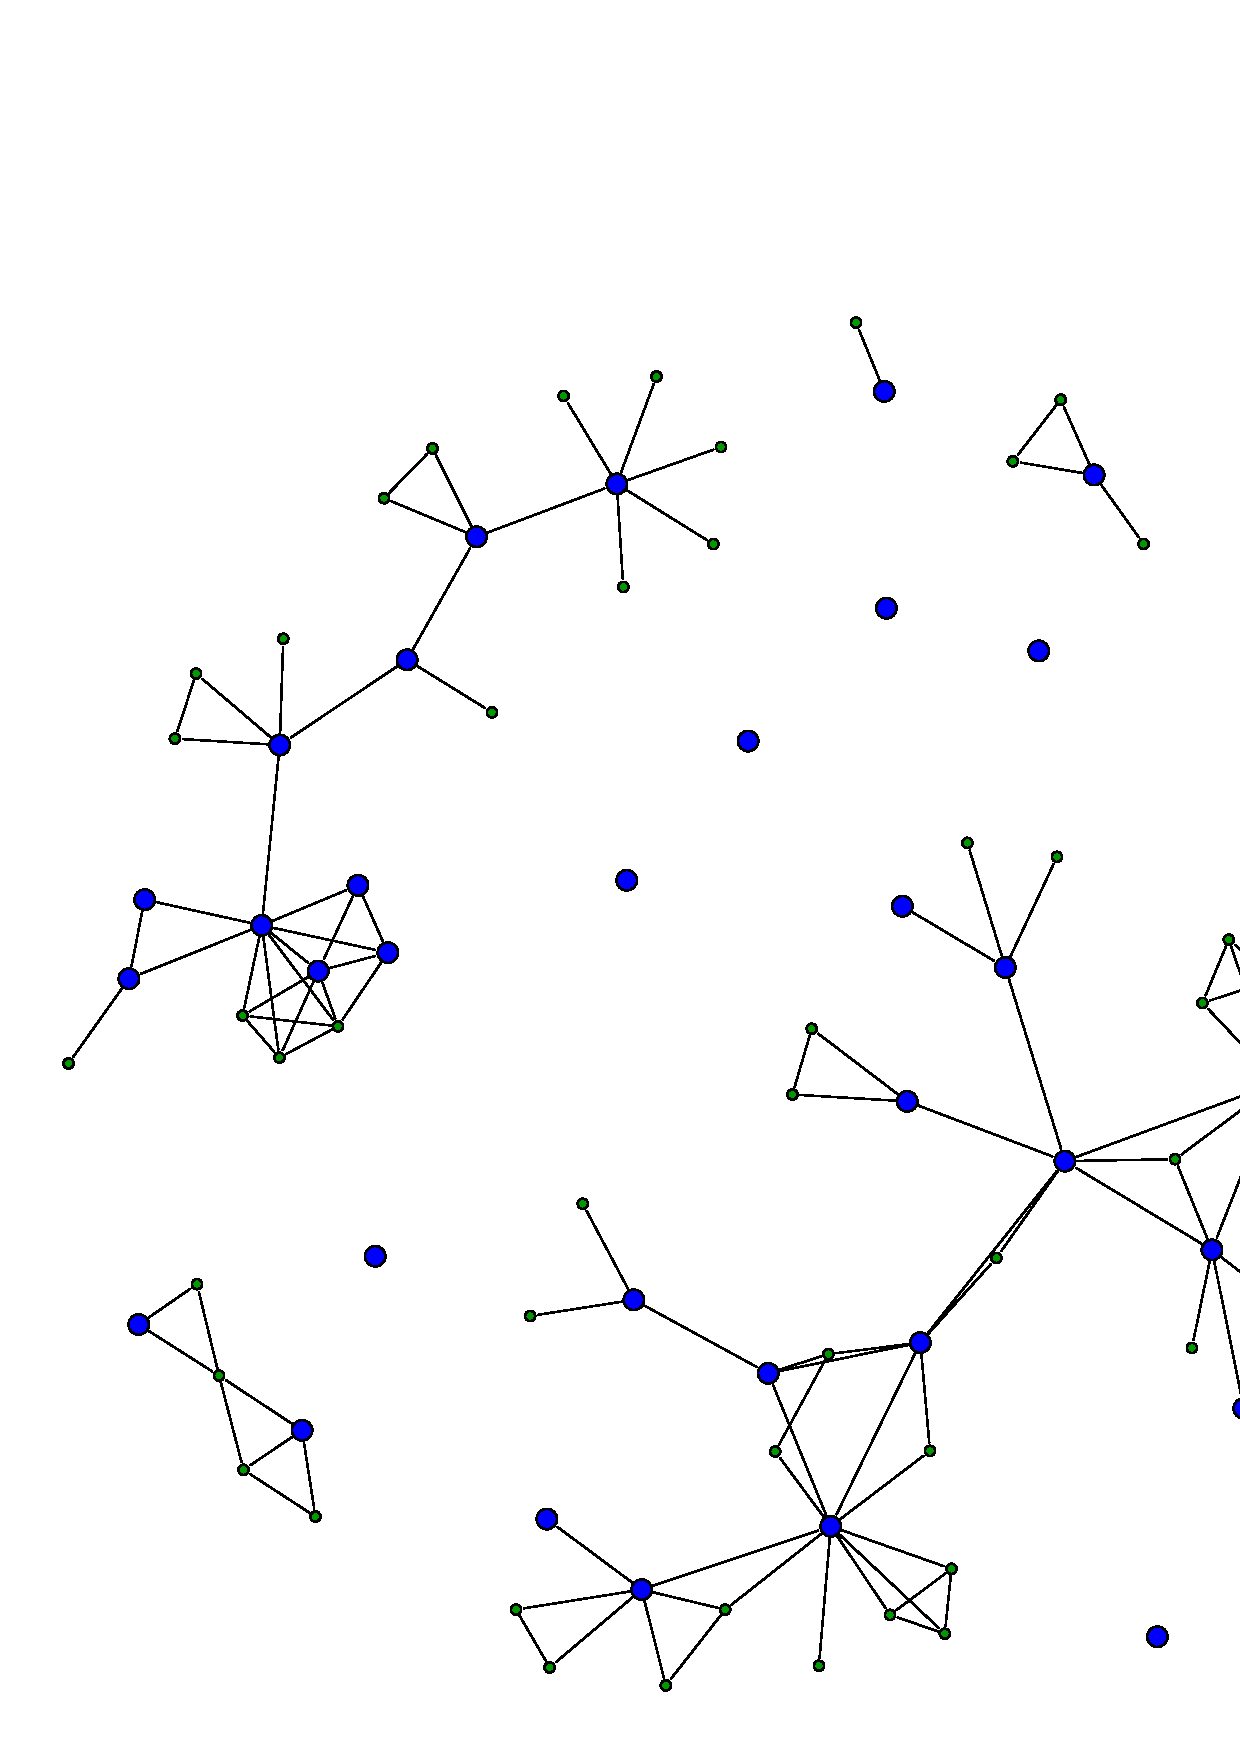
\includegraphics[width=.7\textwidth]{graph}
    \end{turn}
    \caption{O mesmo exemplo, girado.}
    \label{fig:subfigures:b}
  \end{subfigure}

  \caption{Exemplo de subfiguras.}
  \label{fig:subfigures}
\end{figure}

% Foi utilizado o pacote listings para formatar o código fonte
% Veja no preambulo do arquivo tese-exemplo.tex os parâmetros de configuração.
\begin{program}
  \index{Java}
  \centering

\begin{lstlisting}[language=Java, style=wider]
for (i = 0; i < 20; i++)
{
	// Comentário
	System.out.println("Mensagem...");
}
\end{lstlisting}

  \caption{Exemplo de laço em Java.}
  \label{prog:java}
\end{program}

\begin{figure}
  \centering

  \begin{ganttchart}{2017-11}{2018-5}
    \gantttitlecalendar{year,month=shortname} \ganttnewline

    \ganttgroup[progress=45]{Experimento}{2017-11}{2018-2} \ganttnewline
    \ganttbar[progress=100]{
      Preparação\ganttalignnewline
      (compra de insumos)
      }{2017-11}{2017-12} \ganttnewline
    \ganttbar[progress=30]{Execução}{2017-12}{2018-1} \ganttnewline
    \ganttbar[progress=0]{Análise}{2017-12}{2018-2} \ganttnewline

    \ganttgroup[progress=0]{Artigo}{2018-1}{2018-4} \ganttnewline
    \ganttbar[progress=0]{Escrita}{2018-1}{2018-3} \ganttnewline
    \ganttbar[progress=0]{Revisão}{2018-3}{2018-4} \ganttnewline

    \ganttmilestone{Submissão}{2018-4}
  \end{ganttchart}

  \caption{Exemplo de cronograma.}
  \label{fig:gantt}
\end{figure}

Talvez você precise organizar a apresentação da informação na forma de
tabelas\index{Floats}. Há diversos estilos de tabela; um exemplo simples é a
Tabela~\ref{tab:amino_acidos}. A Tabela~\ref{tab:ficha} mostra como construir
uma tabela em forma de ficha larga que deve ser impressa em modo paisagem (ela
é um \textit{float}, mas sempre é impressa em uma página separada). Outro
exemplo de tabela em modo paisagem, esta distribuída em duas páginas (sem ser
um \textit{float}), está no Apêndice \ref{ape:sequencias}\footnote{
Observe que o nome do Apêndice (``\ref{ape:sequencias}'') foi impresso em uma
linha separada, o que não é muito bom visualmente. Para evitar que isso
aconteça (não só no final do parágrafo, mas em qualquer quebra de linha),
faça o que já foi discutido na Seção~\ref{orphanchar} sobre símbolos
matemáticos: utilize um espaço não-separável para fazer referências a
figuras, tabelas, seções etc.: ``\textsf{... está no
Apêndice\textasciitilde\textbackslash{}ref\{ape:sequencias\}}''.}.

\begin{table}
\centering

  \hspace*{\fill}
  \begin{subtable}[b]{0.42\textwidth}
    \centering
    \begin{tabular}{ccl}
      \toprule
      Código      & Abreviatura  & \makecell{Nome\\completo} \\
      \midrule
      \texttt{A}  & Ala          & Alanina \\
      \texttt{C}  & Cys          & Cisteína \\
      ...         & ...          & ... \\
      \texttt{W}  & Trp          & Triptofano \\
      \texttt{Y}  & Tyr          & Tirosina \\
      \bottomrule
    \end{tabular}
    \caption{Uma tabela simples.}
  \end{subtable}
  % Como mencionado mais acima, não deixe linhas em branco aqui
  \hspace*{\fill}\hspace*{\fill}\hspace*{\fill}
  \begin{subtable}[b]{0.37\textwidth}
    \centering
    \begin{tabular}{ccl}
      \rothead{Código} & \rothead{Abreviatura} & \rothead{Nome\\completo} \\
      \midrule
      \texttt{A}       & Ala                   & Alanina \\
      \texttt{C}       & Cys                   & Cisteína \\
      ...              & ...                   & ... \\
      \texttt{W}       & Trp                   & Triptofano \\
      \texttt{Y}       & Tyr                   & Tirosina \\
      \bottomrule
    \end{tabular}
    \caption{Com cabeçalhos girados.}
  \end{subtable}
  \hspace*{\fill}

  \caption{Códigos, abreviaturas e nomes dos aminoácidos.}
  \label{tab:amino_acidos}
\end{table}

% Aumenta o espaçamento entre as linhas da tabela (default: 0pt)
\setlength\extrarowheight{4pt}

% sidewaystable e comandos relacionados são definidos na package rotating
\begin{sidewaystable}
\centering

\begin{tabular}{|M{0.265}|M{0.073}|M{0.084}|M{0.073}|M{0.073}|M{0.08}|M{0.082}|M{0.067}|}
  \hline
    \textbf{Experimento número:} & \multicolumn{2}{c|}{1} & \multicolumn{4}{c|}{\textbf{Data:}} & jan 2017
  \tabularnewline \hline
    \textbf{Título:} & \multicolumn{7}{c|}{Medições iniciais}
  \tabularnewline \hline
    \textbf{Tipo de experimento:} & \multicolumn{7}{c|}{Levantamento quantitativo}
  \tabularnewline \hline \hline
    \textbf{Locais}          & São Paulo & Rio de Janeiro & Porto Alegre & Recife & Manaus & Brasília & Rio Branco
  \tabularnewline \thickhline
    \textbf{Valores obtidos} & 0.2       & 0.3            & 0.2          & 0.7    & 0.5    & 0.1      & 0.4
  \tabularnewline \hline
\end{tabular}

\caption{Exemplo de tabela similar a uma ficha.}
\label{tab:ficha}
\end{sidewaystable}

% Redefinindo para o valor default
\setlength\extrarowheight{0pt}
